\chapter{Experimental Methods}
The data used in this thesis stems from an experiment carried out at the IGISOL facility, at the University of Jyväskylä. Originally the experiment was scheduled for May 2020, but was postponed due to the ongoing Corona pandemic. 


\section{Detector setup}
The detection setup consists of 6 double sided silicon detectors (DSSD), and 6 single sided silicon detectors (SSD). 
The detectors are $\SI{5}{cm} \times \SI{5}{cm}$ and placed in a cube around the a target in the center, as shown on figure \ref{fig}. The setup is designed with measuring the opening angle of the $\beta$ in mind, and therefore the detectors covers 51\% of the solid angle. \\
 

\section{Experimental setup}
The setup is designed to measure $\beta\alpha$ angular correlations in the $\beta$-delayed particle decay of \isotope[8][]{Li}. When measuring multiple particles, the setup is highly dependent on the coverage of the solid angle. Therefore the setup is designed to have a large solid angle coverage, with high $\alpha$-particle resolution, while still being able to measure $\beta$-particles. \\
This is has been achieved by creating a cube of six double sided silicon detectors (DSSD), all backed by a \SI{1}{mm} single sided detector (SSD). To gain the largest solid angle, the detectors where placed as close to one another as possible. A 3D printed case was designed to hold the detectors in place, and achieved a solid angle coverage of 51\% for the DSSD's. An illustration of the setup, together with the different detectors' thickness can be seen on figure \ref{fig:opstilling}. 
Even though the setup was designed to hold 12 detectors in total, there where only 11 detectors in the actual experiment. This was due to one of the SSD's being defect, so it was removed from the setup. 

\begin{figure}[h]
	\fbox{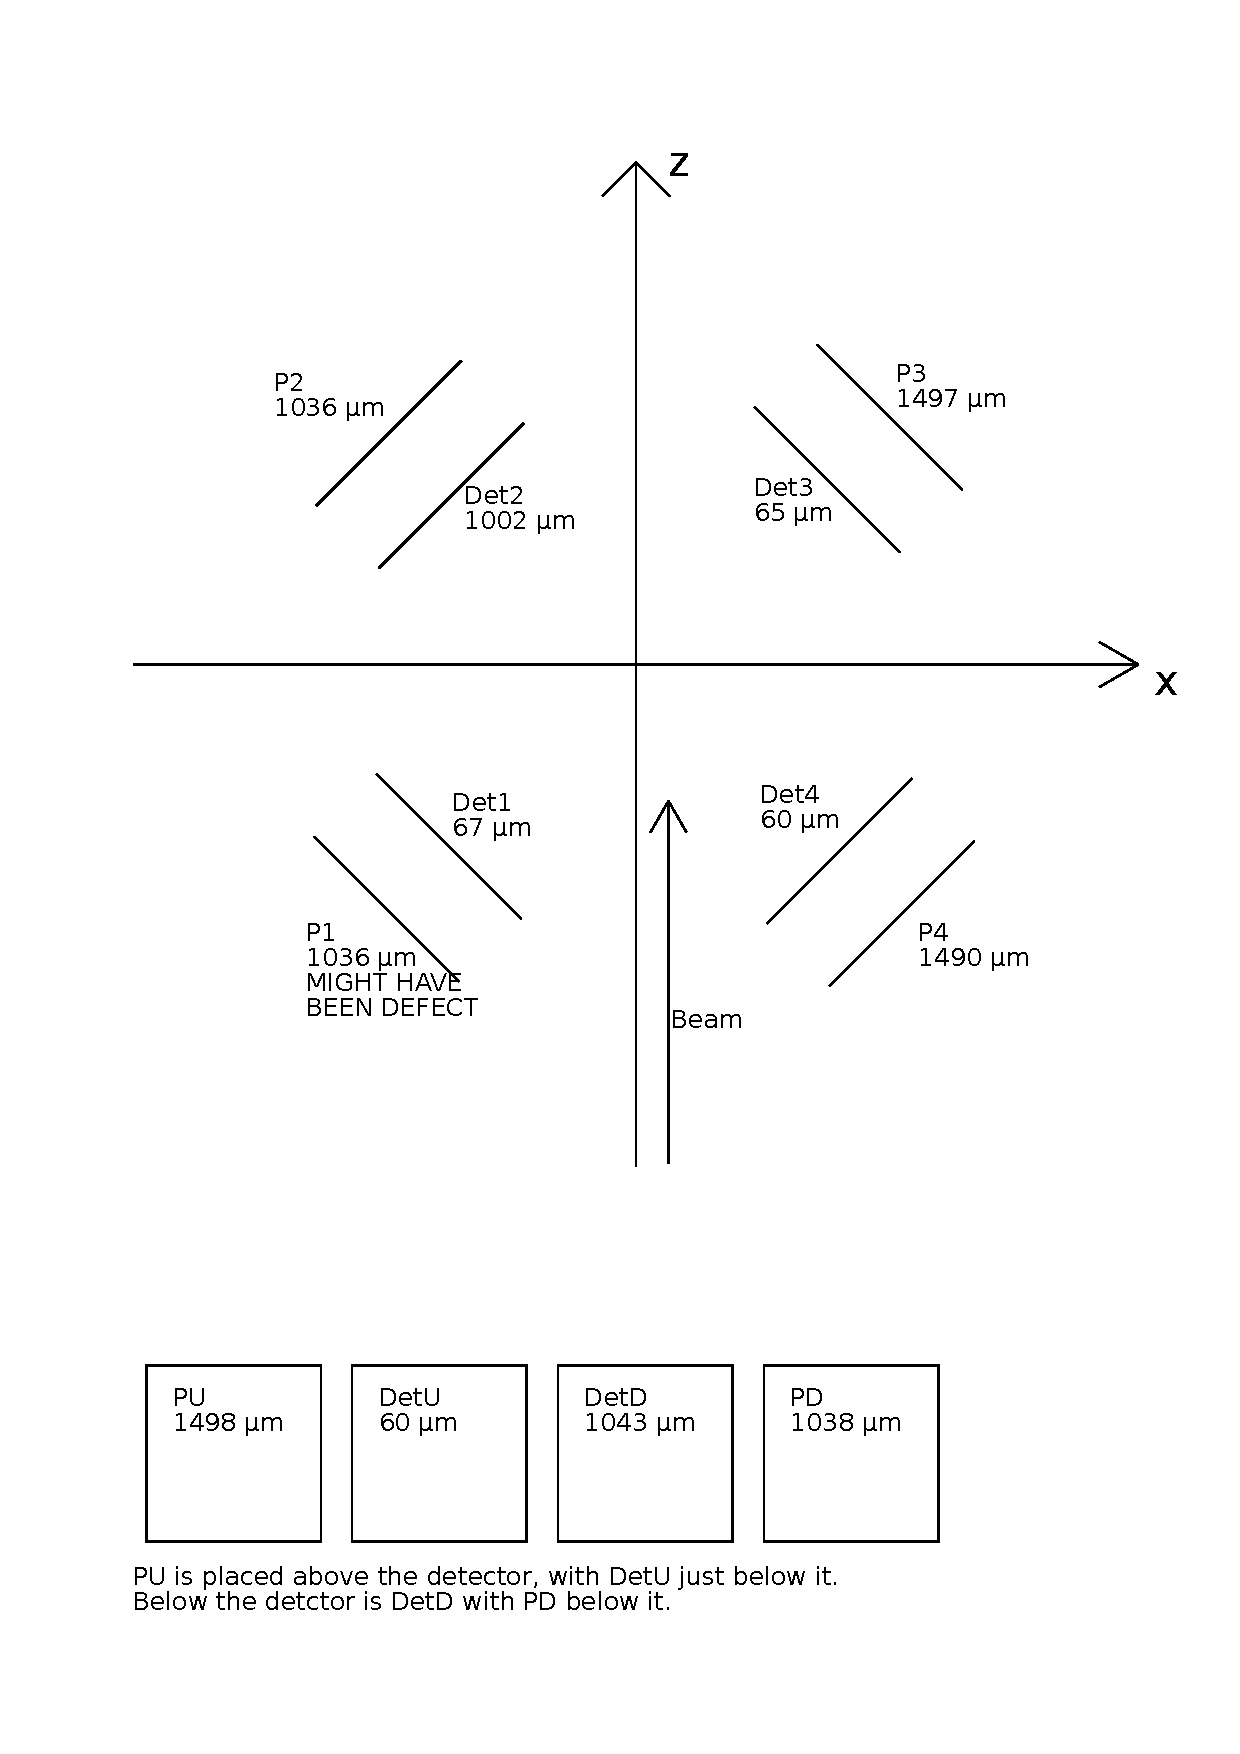
\includegraphics[width=\linewidth]{../figures/opstilling.pdf}}
	\caption{illustration of the setup. Note that the SSD P1 was absent from the actual experiment, due to failure in the detector}
	\label{fig:opstilling}
\end{figure}

\section{The detectors}
As mentioned above, there where two types of detectors present in the setup. The first type is the Double sided silicon detector. 
As the name suggests, it consists of two sides, a front layer and a back layer. Each layer consists of 16 strips, that are placed in rows next to each other. The two layers are then arranged so each side are mutually orthogonal, which defectively makes pixels where each strip intersects a strip on the other side. \\
The strips on the front side are p-doped, while the back side are n-doped. When a charged particle hits the detector, it will ionize the atoms in the semi-conductor, and produce a electron-hole pair. The number of electron-hole pairs is proportional to the energy of the charged particle. 
The bias voltage on the detector collects the electrons and holes on opposite sites of the strip, where the charge is collected on aluminum contacts and a signal is measured. Energy is not deposited in these contacts, and therefore they constitute to a so called dead layer. \\
The detectors are square $5\times 5$ \SI{}{cm} and with their $16\times 16$ strips, they have an effective gird of  256 pixels of \SI{9}{mm}. 
4 of the 6 detectors have a thickness of \SI{60}{\mu m} and a dead layer of \SI{100}{nm} dead layer. These detectectors are the ones called Det1, Det3, Det4 and DetU in the setup seen on figure \ref{fig:opstilling}. The other 2 detectors (Det2 and DetD) where both \SI{1}{mm}.
\\
\\
The other type of detector was the SSD's also known as pads. They are different from the DSSD's, in that they only have one side, and no strips. Therefore they do not contain a grid, the same way the DSSD's do, and will therefore not provide any information as to where on the detector a particle has hit. But the reason they are in this setup, is because they are thicker. They are used to measure the energy deposited by a $\beta$-particle, and to determine if a given particle is a $\beta$-particle. An $\alpha$-particle will deposit all of its energy into the first DSSD it encoutner, and be effectively stopped compleatly by it. But a $\beta$-particle will deposit allmost no energy in a thin DSSD, and travel through it, ending up depositing some energy in the SSD. \\
Therefore one can roughly distinguish the $\alpha$-particles from the $\beta$-particles, by observing wether a particle has a hit in the DSSD and the SSD. \\
\\
Since there are also two thick DSSD's in the setup, one can also get some information from a $\beta$-particle from these thicker detectors, as it will deposit more energy in these detectors. 




\section{AUSAlib and ROOT}
ROOT is an object oriented C++ framework that is designed primarily for data analysis in high-energy and nuclear physics. It was created at CERN in 1995, and has since grown and become the dominant analysis software at both CERN and many other nuclear and particle physics laboratories. 
ROOT was designed to handle large amounts of data with high computing efficiency. \\
ROOT makes an intelligent data structure by creating a "Tree" with the class \texttt{TTree}. This tree will then have "branches" which corresponds to some variable of the given detection event, such as the energy of the front strip or identity of the detector. This TTree then allows for reading of an individual branch, while ROOT takes care of the memory management. One can also store a TTree to the disk in the form a .root file. \\

ASUALib is a tool that build on top of ROOT. It was created by the subatomic group at Aarhus University.
Before this tool was created, everyone in the group had to more or less create their own tools to get data from the detectors into a useful data structure. This meant that a lot of time was wasted just trying to access data from experiments. AUSAlib was therefore created, so the basic tasks of data extraction was automated. \\
AUSAlib has a lot of functionalities, but there are \textcolor{red}{XX} tools that was used in this thesis, namely the \textit{Sorter}, \textit{Calibrator} and the \textit{AbstractSortedAnalyzer}.

\subsection{Calibrator}
Since the detectors work, by measuring an electrical charge that comes from the charged particle, the detectors needs to translate a specific charge to energy deposited. \\
To do that, we use the \texttt{Calibrator}-tool, which is designed to convert a channel number into an actual energy. Assuming that the channel numbers are linearly related to the energies, a known radioactive source can be measured, and the expected spectrum can be compared to the measured. This is done for each strip in each detector.
\\
\\
The \texttt{Calibrator} starts by running a peak-finding algorithm over some calibration data, to roughly identify the locations of the peaks, followed by a multi-Gaussian fit to find the most precise peak location. 
The positions of the peaks can then be compared to the expected energies, giving an associated energy to a given channel. \\
\\
As mentioned earlier, all of the detectors have a small aluminum dead layer. All particles that pass through this layer will loses some amount of energy depending on the stopping power of the material and the effective thickness of the dead layer $\Delta x_{eff}$, which furthermore depends on the angle of incidence, $\theta$. 
The relationship between the effective thickness and the actual thickness is described as $\Delta x_{eff} = \Delta x/ \cos(\theta)$. This gives the measured energy as 
\begin{equation*}
E' = E - \dfrac{dE}{dx} \dfrac{\Delta x}{\cos(\theta)},
\end{equation*}
where $E$ is the original energy of the particle, $dE/dx$ is the stopping power of the material and $\Delta x$ is the thickness of the dead layer. \\
\\
These calculations are all handled by the \texttt{Calibrator}. 
As input it takes an unpacked measurement of a source, a file specifying the locations of the expected peaks and a file specifying the spacial locations of the detectors. 
From this it calculates the energy loss, and creates a linear relationship between channel numbers and energies. This is then written to the disk as a seperate calibration file, which can be parsed to other moduels.\\
It is important to note that the Calibrator does not modify any data. Therefore the energy loss is unaccoutned for. Instead it corrects the expected energy spectrum, which means that the resulting calibration is still valid. The energy loss correction is therefore still needed in the analysis, as the effect is unaccounted for in measurements. 
